\documentclass[letterpaper,11pt]{article}

\usepackage[empty]{fullpage}
\usepackage{titlesec}
\usepackage{enumitem}
\usepackage[hidelinks]{hyperref}
\usepackage{fancyhdr}
\usepackage[english]{babel}
\usepackage{fontawesome}
\usepackage{geometry}
\usepackage[usenames,dvipsnames]{xcolor}
\usepackage{graphicx}

%---------- FONT OPTIONS ----------

\pagestyle{fancy}
\fancyhf{}
\fancyfoot{}
\renewcommand{\headrulewidth}{0pt}
\renewcommand{\footrulewidth}{0pt}

% Adjust margins
\addtolength{\oddsidemargin}{-0.5in}
\addtolength{\evensidemargin}{-0.5in}
\addtolength{\textwidth}{1in}
\addtolength{\topmargin}{-.5in}
\addtolength{\textheight}{1.0in}

\urlstyle{same}

\raggedbottom
\raggedright
\setlength{\tabcolsep}{0in}

\definecolor{LightBlue}{RGB}{173,216,230} 
\titleformat{\section}{
  \vspace{-4pt}\scshape\raggedright\large
}{}{0em}{}[\color{LightBlue}{\titlerule[4pt]} \vspace{-5pt}]

%-------------------------
% Custom commands

\newcommand{\resumeItem}[1]{
  \item\small{
    {#1 \vspace{-2pt}}
  }
}

\newcommand{\resumeSubheading}[4]{
  \vspace{-2pt}\item
    \begin{tabular*}{0.97\textwidth}[t]{l@{\extracolsep{\fill}}r}
      \textbf{#1} & #2 \\
      \textit{\small#3} & \textit{\small #4} \\
    \end{tabular*}\vspace{-7pt}
}

\renewcommand\labelitemii{$\vcenter{\hbox{\tiny$\bullet$}}$}

\newcommand{\resumeSubHeadingListStart}{\begin{itemize}[leftmargin=0.15in, label={}]}
\newcommand{\resumeSubHeadingListEnd}{\end{itemize}}
\newcommand{\resumeItemListStart}{\begin{itemize}}
\newcommand{\resumeItemListEnd}{\end{itemize}\vspace{-5pt}}


%-------------------------------------------
%%%%%%  RESUME STARTS HERE  %%%%%%%%%%%%%%%%%%%%%%%%%%%%

\begin{document}

%---------- HEADING ----------

\noindent
\begin{minipage}[c]{0.3\textwidth}
    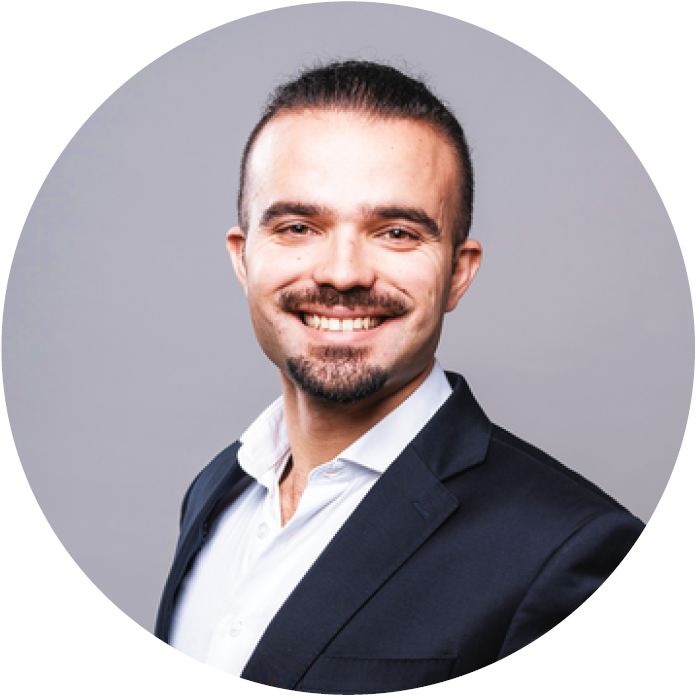
\includegraphics[width=\linewidth]{CV_Picture.png}
\end{minipage}
\hfill
\begin{minipage}[c]{0.65\textwidth}
    \begin{center}
        \textbf{\Huge \scshape Sérgio Tiago Matias}\\[3pt]
        \vspace{4pt}
        \faMapMarker \hspace{.5pt} \href{https://www.google.com/maps/place/Munich/@48.1549958,11.4594364,12z/data=!3m1!4b1!4m6!3m5!1s0x479e75f9a38c5fd9:0x10cb84a7db1987d!8m2!3d48.1351253!4d11.5819805!16s%2Fm%2F02h6_6p?entry=ttu}{Munich, Germany}\\
        \vspace{4pt}
        {\faMobile \hspace{.5pt} \href{tel:01795286313}{+49 (0) 179 5286313}}\\
        \vspace{4pt}
        {\faAt \hspace{.5pt} \href{mailto:sergio.tiago.matias@gmail.com}{sergio.tiago.matias@gmail.com}}\\
        \vspace{4pt}
        \faLinkedinSquare \hspace{.5pt} \href{https://linkedin.com/in/sergiotiagomatias}{LinkedIn}\\
        \vspace{4pt}
        \faGithub \hspace{.5pt} \href{https://github.com/chiefmatias}{GitHub}
    \end{center}
\end{minipage}

%----------- Summary -----------

\section{Summary}
    Unique background in earth sciences, now transitioning to software development. Experienced in managing large-scale data and bridging the gap between technical and non-technical stakeholders. Ability to quickly adapt and excel in intellectually demanding environments exemplified by academic journey. \\ \vspace{3pt}
    
%----------- WORK EXPERIENCE -----------

\section{Work Experience}
  \vspace{2pt}
  \resumeSubHeadingListStart

    \resumeSubheading
       {Personal Development}{Munich, Germany}
       {Software Development}{Jun 2023 \textbf{--} Present}
    \resumeItemListStart
		\resumeItem{\textbf{Deutschkurs (B1):} Attending a semi-intensive German language course to achieve B1 proficiency.}
        \resumeItem{\textbf{Developed a Multi-Component SaaS System:} Engineered a fully automated, event-driven transcription system, leveraging AWS cloud services for robust and scalable hosting (demo on request).}
        \resumeItem{\textbf{Advanced Computing Concepts:} Delved into "Design Patterns: Elements of Reusable Object-Oriented Software" to deepen understanding of advanced design patterns and applied these concepts to Python development.}
        \resumeItem{\textbf{Advanced Networking Knowledge:} Completed "The Bits and Bytes of Computer Networking," an in-depth online course, to reinforce and expand my foundational understanding of computer networking principles and practices.}
         \resumeItemListEnd

     \resumeSubheading
       {NavVis}{Munich, Germany}
       {Data Operations Engineer}{Apr 2021 -- Jun 2023, WS + Full Time}
    \resumeItemListStart
        \resumeItem{Led the development of a user-friendly interface application that simplifies interaction with product's API, enabling non-technical team members to access and utilize data more efficiently. Built with kivy and hosted on remote machines.}
        \resumeItem{Automated two complex workflows, establishing a new standard for the Enterprise team and effectively shortening default deadlines by an average of one working week.}
        \resumeItem{Designed and implemented interim solutions for various client-specific needs, primarily addressing challenges in data flow pipelines and product API integration.}
        \resumeItem{Technical project manager of large enterprise customer (+2M sqm project).}
        \resumeItemListEnd
         
     \resumeSubheading
       {Ludwig-Maximilians-Universität München}{Washington, United States of America}
       {Research Assistant}{Sep 2022 \textbf{--} Oct 2022, Contract}
         \resumeItemListStart
             \resumeItem{Project: "Probing the 4D evolution of active magmatic systems through magnetotelluric monitoring."}
             \resumeItem{Successfully planned and executed a 7-week magnetotellurics field campaign in Mt. St. Helens, WA, including data acquisition and onsite quality control.}
         \resumeItemListEnd

         
     \resumeSubheading
       {Eurofins Genomics}{Ebersberg, Germany}
       {Laboratory Assistant}{Dec 2020 \textbf{--} Mar 2021, Part Time}
         \resumeItemListStart
             \resumeItem{Complied with stringent quality control protocols in accordance with ISO/IEC 17025 standards, governmental regulations, and company-specific requirements.}
             \resumeItem{Executed a range of precise laboratory tasks including sample verification, tube extraction, and pipetting, ensuring accuracy in batch IDs and sample plates.}
         \resumeItemListEnd

    
    \resumeSubheading
      {University of Évora}{Évora, Portugal}
      {Research Assistant}{Jan 2019 \textbf{--} Aug 2019, Internship}
        \resumeItemListStart
            \resumeItem{Project: "Project FIRE- Fogo Island volcano: multi disciplinary Research on 2014 Eruption."}
            \resumeItem{Established and managed a comprehensive seismic database exceeding 2TB, involving organization and curation of large-scale seismic data.}
            \resumeItem{Contributed to various research initiatives within the geophysics and geology departments, providing essential data analysis, experimental design, and fieldwork support.}
        \resumeItemListEnd


%    \resumeSubheading
%      {Private $|$ Study Centers}{Lisbon, Portugal}
%      {Tutor}{2017 \textbf{--} 2019, Part Time}
%        \resumeItemListStart
%            \resumeItem{Geography and English tutoring.}
%            \resumeItem{Private mentoring of two students, 8º and 11º grade.}
%            \resumeItem{Solo and group tutoring in two different study centers.}
%        \resumeItemListEnd
%    
    \resumeSubHeadingListEnd


%----------- EDUCATION -----------

\section{Education}
  \vspace{2pt}
  \resumeSubHeadingListStart
    
    \resumeSubheading
      {Ludwig Maximilian University of Munich
      }{Munich, Germany}
      {M.Sc. in Geophysics;   \textbf{Avg Grade: 3.09} }{2019 \textbf{--} 2022}

    \resumeSubheading
      {University of Lisbon
      }{Lisbon, Portugal}
      {B.Sc. in Geography;   \textbf{Avg Grade: 2.1} }{2015 \textbf{--} 2018}

  \resumeSubHeadingListEnd



%----------- SKILLS -----------

\section{Skills}
  \vspace{2pt}
  \resumeSubHeadingListStart
    \small{\item{
        
    \textbf{Programming Languages:} Python, Shell, C (familiar), JavaScript (basic). \\ \vspace{3pt}
    \textbf{Libraries:} Pandas, NumPy, Matplotlib, Kivy, GeoPandas, Arcpy, GDAL. \\ \vspace{3pt}
    \textbf{Web Development:} Flask, HTML, CSS, Bootstrap. \\ \vspace{3pt}
    \textbf{Databases:} SQLite, PostgreSQL. \\ \vspace{3pt}
    \textbf{Cloud:} S3, Lambda, EC2, RDS, IAM , SES. \\ \vspace{3pt}
    \textbf{DevOps/Tools:} Git, Docker, Linux, Boto3 (Python AWS SDK), RabbitMQ, GitHub Actions. \\ \vspace{3pt}
    
    }}
    
  \resumeSubHeadingListEnd

%----------- Languages -----------

\section{Languages}
  \vspace{2pt}
  \resumeSubHeadingListStart
    \small{\item{
        
    \textbf{Portuguese:} Native \\ \vspace{3pt}
    \textbf{English:} Fluent \\ \vspace{3pt}
    \textbf{Spanish:} Advanced \\ \vspace{3pt}
    \textbf{German:} Basic \\ \vspace{3pt}
    
    }}
  
  \resumeSubHeadingListEnd


%----------- OTHER -----------

 \section{Other}
   \vspace{2pt}
   \resumeSubHeadingListStart
    \small{\item{
         \textbf{Geonatura GIS Course:} Achieved top rank with the highest grade in a cohort of 20 students. Awarded a full scholarship for further studies at Delft University of Technology. (2019)} \\ \vspace{3pt}
    
         \textbf{Conferences:} Participated in "Jornadas do ICT" and the "11th APMG Meteorology and Geophysics Symposium." Presented posters titled "Lava Flow Modeling at Pico Island" and "CEG's Mission during the 1957 Eruption of Capelinhos." (2019)} \\ \vspace{3pt}

   \resumeSubHeadingListEnd


\end{document}